\section{Ramsey Growth Model}

\begin{frame}

\begin{center}
{\LARGE Ramsey Growth Model}
\end{center}

\end{frame}

%------------------------------------------------
%------------------------------------------------

\begin{frame}{Ramsey model}

Production economy, rather than endowment
\begin{itemize}
\item Log utility
\item Labor supply exogenous (constant and normalized to unity)
\item Constant returns to scale in production function
\item $100\%$ depreciation of capital (`investment' in $t$ = $K_{t+1}$)
\item Technology, $\theta_{t}$, grows at rate $g$
\item Infinitely-lived \textit{representative} agent
\end{itemize}

\end{frame}

%------------------------------------------------
%------------------------------------------------

\begin{frame}{Household problem in Ramsey}

Representative household maximizes lifetime utility
\begin{gather*}
\underset{\{C_{t+s},K_{t+s+1}\}}{\max }\underset{s=0}{\overset{\infty }{\sum}}\beta ^{s}\log C_{t+s} \\
\text{s.t.} \\
K_{t+s+1}=r_{t+s}K_{t+s}+w_{t+s}- C_{t+s} \; \forall s\geq 0 \\
K_{t}\text{ given,} \\
\underset{T\rightarrow \infty }{\lim }\frac{K_{T+1}}{\tilde{R}_{T}}\geq 0
\end{gather*}

Euler equation for consumption as before
\begin{equation*}
\frac{C_{t+1}}{\beta C_{t}}=r_{t+1}
\end{equation*}

\end{frame}

%------------------------------------------------
%------------------------------------------------

\begin{frame}{Household problem in Ramsey}

Representative household maximizes lifetime utility
\begin{gather*}
\underset{\{C_{t+s},K_{t+s+1}\}}{\max }\underset{s=0}{\overset{\infty }{\sum}}\beta ^{s}\log C_{t+s} \\
\text{s.t.} \\
\overbrace{K_{t+s+1}}^{Investment}=\overbrace{\underbrace{r_{t+s}K_{t+s}+w_{t+s}}_{Earnings}- C_{t+s}}^{Savings} \; \forall s\geq 0 \\
K_{t}\text{ given,} \\
\underset{T\rightarrow \infty }{\lim }\frac{K_{T+1}}{\tilde{R}_{T}}\geq 0
\end{gather*}

Euler equation for consumption as before
\begin{equation*}
\frac{C_{t+1}}{\beta C_{t}}=r_{t+1}
\end{equation*}

\end{frame}

%------------------------------------------------
%------------------------------------------------

\begin{frame}{Household problem in Ramsey}

Representative household maximizes lifetime utility
\begin{gather*}
\underset{\{C_{t+s},K_{t+s+1}\}}{\max }\underset{s=0}{\overset{\infty }{\sum}}\beta ^{s}\log C_{t+s} \\
\text{s.t.} \\
K_{t+s+1}=r_{t+s}K_{t+s}+w_{t+s} \textcolor{red}{\underbrace{L_{t}^{S}}_{\equiv 1}}- C_{t+s} \; \forall s\geq 0 \\
K_{t}\text{ given,} \\
\underset{T\rightarrow \infty }{\lim }\frac{K_{T+1}}{\tilde{R}_{T}}\geq 0
\end{gather*}

Euler equation for consumption as before
\begin{equation*}
\frac{C_{t+1}}{\beta C_{t}}=r_{t+1}
\end{equation*}

\end{frame}

%------------------------------------------------
%------------------------------------------------

\begin{frame}{Firm problem in Ramsey}

Firm maximizes profits
\begin{equation*}
\underset{K_{t},L^{D}_{t}}{\max }\left( K_{t}^{\alpha }\left( \theta_{t}L^{D}_{t}\right) ^{1-\alpha }-w_{t}L^{D}_{t}-r_{t}K_{t}\right)
\end{equation*}

First order conditions define factor prices as before
\begin{eqnarray*}
r_{t} &=&\alpha K_{t}^{\alpha -1}\left( \theta _{t}L^{D}_{t}\right) ^{1-\alpha }\\
w_{t} &=&\left( 1-\alpha \right) K_{t}^{\alpha }\theta _{t}\left( \theta_{t}L^{D}_{t}\right) ^{-\alpha }
\end{eqnarray*}

\end{frame}

%------------------------------------------------
%------------------------------------------------

\begin{frame}{Firm problem in Ramsey}

Why have I written $L_{t}^{D}$ and $L_{t}^{S}$ rather than $L_{t}$?
\begin{itemize}
\item	$L_{t}^{S}\equiv 1$ isn't important
\item	What \textit{is} important is that outside equilibrium (without appropriate `prices') there's no reason to think $L_{t}^{S}=L_{t}^{D}$
\item	We need $w_{t}$ and $r_{t}$ to (among other things) induce firms to set $L_{t}^{D}$ - thus clearing markets
\end{itemize}

\vspace{1.5mm}
$L_{t}^{S}=L_{t}^{D}$ is an equilibrium condition
\begin{itemize}
\item	Incorporating it allows us to use $L_{t}$ as the amount of labor (supplied and demanded) in equilibrium
\item	I should really be doing this for $K_{t}^{S}$ and $K_{t}^{D}$ but life's too short and typos too numerous\ldots
\end{itemize}

\vspace{1.5mm}
In a price taking world, who sets the prices to the `necessary' values?
\begin{itemize}
\item	Hmmmm,\ldots ponder\ldots
\item	Anyway, regardless, these prices induce an equilibrium
\end{itemize}

\end{frame}

%------------------------------------------------
%------------------------------------------------

\begin{frame}{Equilibrium in Ramsey}

A competitive equilibrium is a sequence 
\begin{equation*}
\left\{ r_{t},w_{t},C_{t},K_{t},L_{t}\right\} _{t=0}^{\infty }
\end{equation*}

s.t.

\begin{enumerate}
\item $\left\{ C_{t},K_{t+1}\right\} $ solves household problem given $\left\{ r_{t},w_{t}\right\} $
\item $\left\{ K_{t},L_{t}\right\} $ solves firm problem given $\left\{r_{t},w_{t}\right\} $
\item Markets clear $L_{t}=1$ and $C_{t}+K_{t+1}=Y_{t}=K_{t}^{\alpha }\left(\theta _{t}L_{t}\right) ^{1-\alpha }$
\item $K_{t}$ given
\item TVC
\end{enumerate}

\end{frame}

%------------------------------------------------
%------------------------------------------------

\begin{frame}{Equilibrium in Ramsey}

Euler equation for consumption and return to capital imply
\begin{equation*}
\frac{1}{C_{t}}=\alpha \beta \frac{1}{C_{t+1}}K_{t+1}^{\alpha -1}\left(\theta _{t+1}L_{t+1}\right) ^{1-\alpha }
\end{equation*}

Substitute in for market clearing conditions and rearrange
\begin{equation*}
\frac{Y_{t+1}}{C_{t+1}}=-\frac{1}{\alpha \beta }+\frac{1}{\alpha \beta } \frac{Y_{t}}{C_{t}}
\end{equation*}

\vspace{2mm}
Only stable solution is $\frac{Y_{t}}{C_{t}} = \frac{1}{1-\alpha \beta} \; \forall t\geq 0$

\end{frame}

%------------------------------------------------
%------------------------------------------------

\begin{frame}{Equilibrium in Ramsey}

\begin{figure}
\centering
\label{fig:ramsey_transversality}
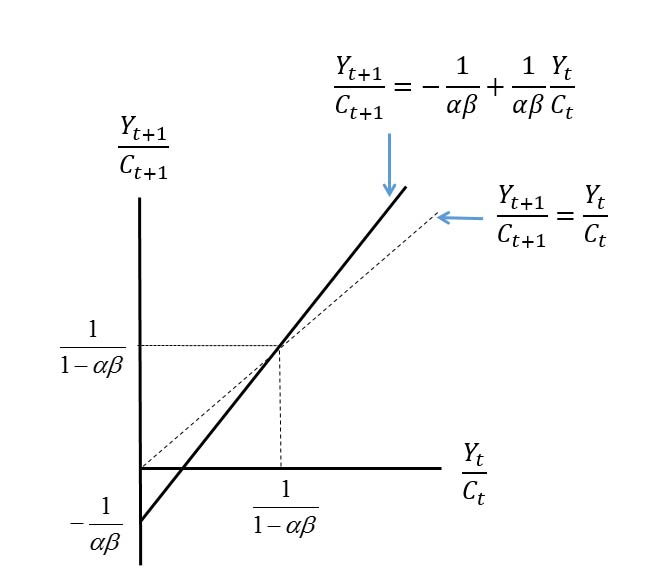
\includegraphics[width=0.6\textwidth]{Figures/ramsey_transversality.JPG}
\end{figure}

Only stable solution is $\frac{Y_{t}}{C_{t}} = \frac{1}{1-\alpha \beta} \; \forall t\geq 0$

\end{frame}

%------------------------------------------------
%------------------------------------------------

\begin{frame}{Equilibrium in Ramsey with technological change}

\begin{itemize}
\item $Y_{t}/C_{t},$ $Y_{t}/K_{t+1}$ constant
\item $\theta _{t},C_{t},K_{t},Y_{t}$ grow at rate $g$
\item $r_{t}=\alpha K_{t}^{\alpha -1}\left( \theta _{t}L_{t}\right)^{1-\alpha }$ $=\alpha \tilde{K}_{t}^{\alpha -1}$ constant
\item $w_{t}=\left( 1-\alpha \right) K_{t}^{\alpha }\theta _{t}\left( \theta_{t}L_{t}\right) ^{-\alpha }=\left( 1-\alpha \right) \theta _{t}\tilde{K}_{t}^{\alpha }$ grows at rate $g$
\end{itemize}

\end{frame}

%------------------------------------------------
%------------------------------------------------

\begin{frame}{Check Kaldor (1957) facts}

\begin{enumerate}
\item Output per worker grows at a roughly constant rate \textcolor{red}{YUP}
\item Capital per worker grows over time \textcolor{red}{YUP}
\item Capital/output ratio is roughly constant \textcolor{red}{YUP}
\item Rate of return to capital is constant \textcolor{red}{YUP}
\item Shares of capital and labor in net income are nearly constant \textcolor{red}{YUP}
\item Real wage grows over time \textcolor{red}{YUP}
\item Ratios of consumption and investment to GDP\ are constant \textcolor{red}{YUP}
\end{enumerate}

\end{frame}

%------------------------------------------------
%------------------------------------------------

\begin{frame}{Endogenous growth models}

Growth is exogenous in this model
	\begin{itemize}
	\item	$\theta_{t}$ an exogenous process
	\end{itemize}
\vspace{2mm}
\textit{Endogenous} growth models seek to explain growth
	\begin{itemize}
	\item	Not covering in depth - but may be in a problem set, say
	\end{itemize}
\vspace{2mm}
\textbf{Extended accumulation} \textbf{models}
	\begin{itemize}
	\item	Overcome diminishing returns to capital by adding externalities in capital accumulation (learning-by-doing and AK model)
	\item	Alternatively, additional factors of production (human capital)
	\end{itemize}
\vspace{2mm}
\textbf{Innovation models}
	\begin{itemize}
	\item	Explain technological progress as a function of endogenous variables
	\item	E.g. Investment in R\&D
	\end{itemize}

\end{frame}

%------------------------------------------------
%------------------------------------------------

\begin{frame}{Growth accounting}

Take logs (see lect. 1) and differentiate $Y_{t}=K_{t}^{\alpha }\left( \theta_{t}L_{t}\right) ^{1-\alpha }$ to decompose into weighted percentage growth rates
\begin{equation*}
\frac{1}{Y_{t}}\frac{dY_{t}}{dt}=\alpha \frac{1}{K_{t}}\frac{dK_{t}}{dt}+(1-\alpha )\frac{1}{\theta_{t}}\frac{d\theta_{t}}{dt}+(1-\alpha )\frac{1}{L_{t}}\frac{dL_{t}}{dt}
\end{equation*}

\vspace{5mm}
Capital share of income in equilibrium$=\alpha$, so set $\approx 1/3$ (as in historical data)
\begin{eqnarray*}
\text{Growth in }Y_{t}\text{ } &=&\frac{1}{3}\times \text{Growth in }K_{t} \\
&&+\frac{2}{3}\times \left( \text{Growth in }\theta _{t}+\text{Growth in }L_{t}\right)
\end{eqnarray*}

\end{frame}

%%------------------------------------------------
%%------------------------------------------------

\begin{frame}{Growth accounting in the $20^{th}$ century, Crafts (2000)}

\begin{figure}
\centering
\subfigure{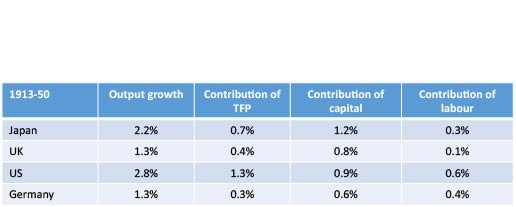
\includegraphics[width=0.45\textwidth]{Figures/growth_1913_50.JPG}}\\
\subfigure{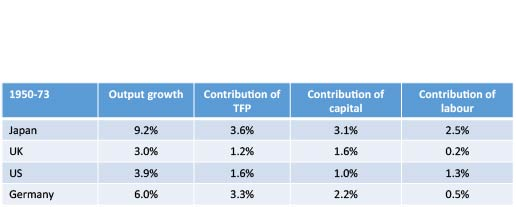
\includegraphics[width=0.45\textwidth]{Figures/growth_1950_73.JPG}}\\
\subfigure{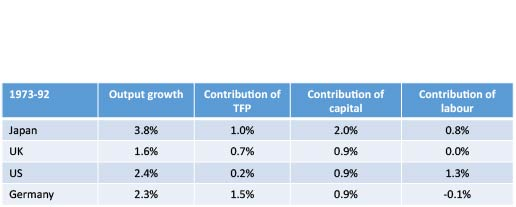
\includegraphics[width=0.45\textwidth]{Figures/growth_1970_92.JPG}}
\end{figure}

\end{frame}

%------------------------------------------------
%------------------------------------------------

\begin{frame}{Growth accounting in emerging markets 1960-1994}
\begin{figure}
\centering
\label{fig:growth_decomp}
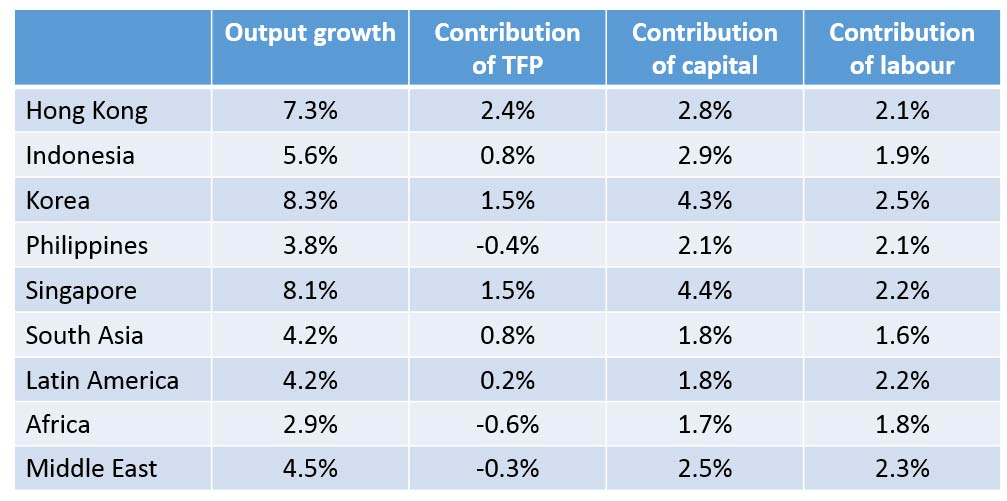
\includegraphics[width=0.8\textwidth]{Figures/growth_decomp.JPG}
\end{figure}
\end{frame}

%------------------------------------------------
%------------------------------------------------

\begin{frame}{Growth accounting for the UK 1970-2013, ONS\ (2015)}

\begin{figure}
\centering
\label{fig:growth_decomp}
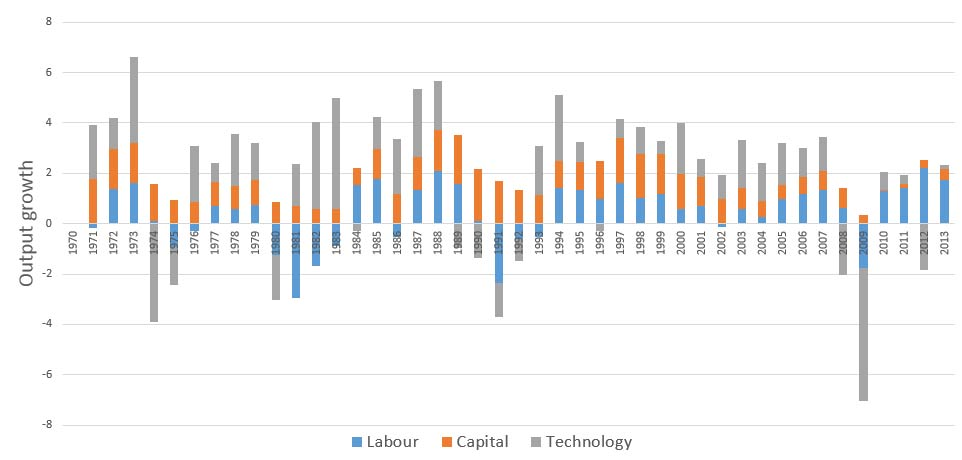
\includegraphics[width=0.8\textwidth]{Figures/growth_decomp_chart.JPG}
\end{figure}

Average UK growth of $2.1\%$
	\begin{itemize}
	\item	$0.4\%$ from technology
	\item	$0.2\%$ from capital
	\item	$0.5\%$ from labor
	\end{itemize}

\end{frame}